\documentclass{standalone}

\usepackage{tikz}
\usepackage{circuitikz}

\tikzset{block/.style = {draw, fill=white, very thick, rectangle, minimum height=1cm, minimum width=2cm},
         lblock/.style={draw,fill=white,very thick, rectangle, minimum height=3cm, minimum width=1cm},
         sum/.style= {draw, fill=white, very thick, circle, node distance=0.5cm}}

         
\begin{document}
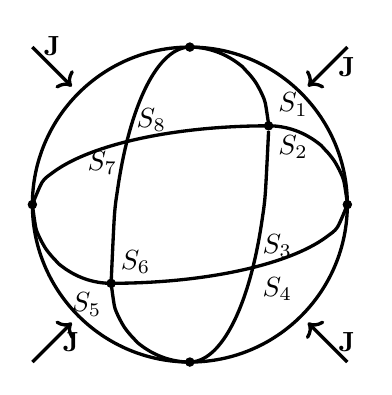
\begin{tikzpicture}[scale=2]
    \draw[very thick](0,0)circle(1);
    \draw[-, very thick]plot[smooth, domain=0.5:1](\x,{(0.25-(\x-0.5)^2)^0.5});
    \draw[-, very thick]plot[smooth, domain=-1:-0.5](\x,{-(0.25-(\x+0.5)^2)^0.5});
    \draw[-, very thick]plot[smooth, domain=-1:0.5](\x,{1/3*(2.25-(\x-0.5)^2)^0.5});
    \draw[-, very thick]plot[smooth, domain=-0.5:1](\x,{-1/3*(2.25-(\x+0.5)^2)^0.5});
    \draw[-, very thick]plot[smooth, domain=-0.5:0](\x,{1/2*(-1+(9-36*(\x)^2)^0.5)});
    \draw[-, very thick]plot[smooth, domain=0:0.5](\x,{1/2*(1-(9-36*(\x)^2)^0.5)});
    \draw[-,very thick]plot[smooth, domain=0:0.5](\x,{(0.25-(\x)^2)^0.5+0.5});
    \draw[-,very thick]plot[smooth, domain=-0.5:0](\x,{-(0.25-(\x)^2)^0.5-0.5});
    
    \draw[<-,very thick](0.75,0.75)--(1,1)node[midway, right]{$\mathbf{J}$};
    \draw[<-,very thick](-0.75,-0.75)--(-1,-1)node[midway, right]{$\mathbf{J}$};
    \draw[<-, very thick](0.75,-0.75)--(1,-1)node[midway, right]{$\mathbf{J}$};
    \draw[<-, very thick](-0.75,0.75)--(-1,1)node[midway, above]{$\mathbf{J}$};

    \filldraw[black](1,0)circle(0.75pt);
    \filldraw[black](-1,0)circle(0.75pt);
    \filldraw[black](0,1)circle(0.75pt);
    \filldraw[black](0,-1)circle(0.75pt);
    \filldraw[black](0.5,0.5)node[above right]{$S_1$}node[below right]{$S_2$}circle(0.75pt);
    \node[above right]at(0.4,-0.4){$S_3$};
    \node[below right]at(0.4,-0.4){$S_4$};
    \filldraw[black](-0.5,-0.5)node[above right]{$S_6$}node[below left]{$S_5$}circle(0.75pt);
    \node[above right]at(-0.4,0.4){$S_8$};
    \node[below left]at(-0.4,0.4){$S_7$};
\end{tikzpicture}
\end{document}